\documentclass [PhD] {uclathes}

% \newcommand{\hvecf}{{\mathbf h}}
\newcommand{\bvecf}{{\mathbf b}}
\newcommand{\pvecf}{{\mathbf p}}
\newcommand{\kvecf}{{\mathbf k}}
\newcommand{\wvecf}{{\mathbf w}}
\newcommand{\nvecf}{{\mathbf n}}
\newcommand{\qvecf}{{\mathbf q}}
\newcommand{\yvecf}{{\mathbf y}}
\newcommand{\cvecf}{{\mathbf c}}
\newcommand{\zvecf}{{\mathbf z}}
\newcommand{\uvecf}{{\mathbf u}}
\newcommand{\vvecf}{{\mathbf v}}
\newcommand{\mvecf}{{\mathbf m}}
\newcommand{\avecf}{{\mathbf a}}
\newcommand{\lvecf}{{\mathbf l}}
\newcommand{\xvecf}{{\mathbf x}}
\newcommand{\Gvecf}{{\mathbf G}}
\newcommand{\dvecf}{{\mathbf d}}
\newcommand{\evecf}{{\mathbf e}}
\newcommand{\tvecf}{{\mathbf t}}
\newcommand{\svecf}{{\mathbf s}}
\newcommand{\rvecf}{{\mathbf r}}
\newcommand{\gvecf}{{\mathbf g}}
%\newcommand{\hvec}{{\mathrm h}}
%\newcommand{\bvec}{{\mathrm b}}
%\newcommand{\pvec}{{\mathrm p}}
%\newcommand{\kvec}{{\mathrm k}}
%\newcommand{\wvec}{{\mathrm w}}
%\newcommand{\nvec}{{\mathrm n}}
%\newcommand{\qvec}{{\mathrm q}}
%\newcommand{\yvec}{{\mathrm y}}
%\newcommand{\cvec}{{\mathrm c}}
%\newcommand{\zvec}{{\mathrm z}}
%\newcommand{\uvec}{{\mathrm u}}
%\newcommand{\vvec}{{\mathrm v}}
%\newcommand{\mvec}{{\mathrm m}}
%\newcommand{\avec}{{\mathrm a}}
%\newcommand{\lvec}{{\mathrm l}}
%\newcommand{\xvec}{{\mathrm x}}
%\newcommand{\dvec}{{\mathrm d}}
%\newcommand{\evec}{{\mathrm e}}
%\newcommand{\tvec}{{\mathrm t}}
%\newcommand{\svec}{{\mathrm s}}
%\newcommand{\rvec}{{\mathrm r}}
%\newcommand{\gvec}{{\mathrm g}}

\newcommand{\hvec}{{h}}
\newcommand{\bvec}{{b}}
\newcommand{\pvec}{{p}}
\newcommand{\kvec}{{k}}
\newcommand{\wvec}{{w}}
\newcommand{\nvec}{{n}}
\newcommand{\qvec}{{q}}
\newcommand{\yvec}{{y}}
\newcommand{\cvec}{{c}}
\newcommand{\zvec}{{z}}
\newcommand{\uvec}{{u}}
\newcommand{\vvec}{{v}}
\newcommand{\mvec}{{m}}
\newcommand{\avec}{{a}}
\newcommand{\lvec}{{l}}
\newcommand{\xvec}{{x}}
\newcommand{\dvec}{{d}}
\newcommand{\evec}{{e}}
\newcommand{\tvec}{{t}}
\newcommand{\svec}{{s}}
\newcommand{\rvec}{{r}}
\newcommand{\gvec}{{g}}
\newcommand{\Gvec}{{\mathrm G}}
\newcommand{\lambdavec}{$$\mbox{\boldmath$\lambda$}$$}
\newcommand{\Thetamat}{{\mathbf \Theta}}
\newcommand{\Phimat}{{\mathbf \Phi}}
\newcommand{\Deltamat}{{\mathbf \Delta}}
\newcommand{\Sigmamat}{{\mathbf \Sigma}}
\newcommand{\Omegamat}{{\mathbf \Omega}}
\newcommand{\Psimat}{{ \Psi}}
\newcommand{\Pimat}{{\mathbf \Pi}}
\newcommand{\Gammamat}{{\mathbf \Gamma }}
\newcommand{\Lambdamat}{{\mathbf \Lambda}}
\newcommand{\epsilonvec}{{\mathbf \epsilon}}
\newcommand{\etavec }{{\mathbf \eta }}
\newcommand{\zeromat }{{\mathbf 0 }}
\newcommand{\Zeromat }{{\mathbf 0 }}
%\newcommand{\log10}{{\log_{10}}}
\newcommand{\Gmat}{{G}}
\newcommand{\Omat}{{O}}
\newcommand{\Mmat}{{M}}
\newcommand{\Lmat}{{L}}
\newcommand{\Emat}{{E}}
\newcommand{\Vmat}{{V}}
\newcommand{\Kmat }{{K}}
\newcommand{\Fmat }{{F}}
\newcommand{\Bmat}{{B}}
\newcommand{\Cmat}{{C}}
\newcommand{\Hmat}{{H}}
\newcommand{\Imat}{{\mathbf I}}
\newcommand{\Dmat}{{D}}
\newcommand{\Qmat}{{Q}}
\newcommand{\Rmat}{{R}}
\newcommand{\Jmat}{{J}}
\newcommand{\Xmat}{{X}}
\newcommand{\Nmat}{{N}}
\newcommand{\Amat}{{A}}
\newcommand{\Ymat}{{Y}}
\newcommand{\Wmat}{{W}}
\newcommand{\Umat}{{U}}
\newcommand{\Tmat}{{T}}
\newcommand{\Smat}{{S}}
\newcommand{\Zmat}{{Z}}
\newcommand{\Pmat}{{P}}
%\newcommand{\Gmat}{{\mathrm G}}
%\newcommand{\Omat}{{\mathrm O}}
%\newcommand{\Mmat}{{\mathrm M}}
%\newcommand{\Lmat}{{\mathrm L}}
%\newcommand{\Emat}{{\mathrm E}}
%\newcommand{\Vmat}{{\mathrm V}}
%\newcommand{\Kmat }{{\mathrm K}}
%\newcommand{\Fmat }{{\mathrm F}}
%\newcommand{\Bmat}{{\mathrm B}}
%\newcommand{\Cmat}{{\mathrm C}}
%\newcommand{\Hmat}{{\mathrm H}}
%\newcommand{\Imat}{{\mathrm I}}
%\newcommand{\Dmat}{{\mathrm D}}
%\newcommand{\Qmat}{{\mathrm Q}}
%\newcommand{\Rmat}{{\mathrm R}}
%\newcommand{\Jmat}{{\mathrm J}}
%\newcommand{\Xmat}{{\mathrm X}}
%\newcommand{\Nmat}{{\mathrm N}}
%\newcommand{\Amat}{{\mathrm A}}
%\newcommand{\Ymat}{{\mathrm Y}}
%\newcommand{\Wmat}{{\mathrm W}}
%\newcommand{\Umat}{{\mathrm U}}
%\newcommand{\Tmat}{{\mathrm T}}
%\newcommand{\Smat}{{\mathrm S}}
%\newcommand{\Zmat}{{\mathrm Z}}
%\newcommand{\Pmat}{{\mathrm P}}
\newcommand{\Gmatf}{{\mathbf G}}
\newcommand{\Omatf}{{\mathbf O}}
\newcommand{\Mmatf}{{\mathbf M}}
\newcommand{\Lmatf}{{\mathbf L}}
\newcommand{\Ematf}{{\mathbf E}}
\newcommand{\Vmatf}{{\mathbf V}}
\newcommand{\Rmatf}{{\mathbf R}}
\newcommand{\Kmatf }{{\mathbf K}}
\newcommand{\Fmatf }{{\mathbf F}}
\newcommand{\Hmatf}{{\mathbf H}}
\newcommand{\Imatf}{{\mathbf I}}
\newcommand{\Dmatf}{{\mathbf D}}
\newcommand{\Qmatf}{{\mathbf Q}}
\newcommand{\Jmatf}{{\mathbf J}}
\newcommand{\Xmatf}{{\mathbf X}}
\newcommand{\Nmatf}{{\mathbf N}}
\newcommand{\Amatf}{{\mathbf A}}
\newcommand{\Ymatf}{{\mathbf Y}}
\newcommand{\Wmatf}{{\mathbf W}}
\newcommand{\Umatf}{{\mathbf U}}
\newcommand{\Tmatf}{{\mathbf T}}
\newcommand{\Smatf}{{\mathbf S}}
\newcommand{\Zmatf}{{\mathbf Z}}
\newcommand{\Pmatf}{{\mathbf P}}
\newcommand{\Bmatf}{{\mathbf B}}
\newcommand{\Cmatf}{{\mathbf C}}
\newcommand{\be }{\begin{equation}}
\newcommand{\ee }{\end{equation}}
\newcommand{\beqn }{\begin{eqnarray}}
\newcommand{\eeqn }{\end{eqnarray}}
                         % personal LaTeX macros
\usepackage{graphicx}
\usepackage{amsmath}
\usepackage{siunitx}
\newcommand{\ud}{\,\mathrm{d}} % "\ud" can be used in mathematical expressions to generate a good differential "d" letter in derivatives and integrals. Here, "\," generates a 3/18 quad space (Width of letter "M").

%%%%%%%%%%%%%%%%%%%%%%%%%%%%%%%%%%%%%%%%%%%%%%%%%%%%%%%%%%%%%%%%%%%%%%
%
% Usually things live in separate flies.
%
% \input {prelim}                           % preliminary page info

%%%%%%%%%%%%%%%%%%%%%%%%%%%%%%%%%%%%%%%%%%%%%%%%%%%%%%%%%%%%%%%%%%%%%%%%
%                                                                      %
%                          PRELIMINARY PAGES                           %
%                                                                      %
%%%%%%%%%%%%%%%%%%%%%%%%%%%%%%%%%%%%%%%%%%%%%%%%%%%%%%%%%%%%%%%%%%%%%%%%

\title          {High-Speed Imaging and Optical Sensing Systems for Biomedical Applications}
\author         {Ata Mahjoubfar}
% Note: department is really your area of research.  I.e. leave out 'Department of'.
\department     {Electrical Engineering}
% Note:  degreeyear should be optional, but as of  5-Feb-96
% it seems required or you get a year of ``2''.   -johnh
\degreeyear     {2014}

%%%%%%%%%%%%%%%%%%%%%%%%%%%%%%%%%%%%%%%%%%%%%%%%%%%%%%%%%%%%%%%%%%%%%%%%

\chair          {Bahram Jalali}
\member         {Benjamin S. Williams}
\member         {Katsushi Arisaka}
\member         {Kayvan Niazi}
\member         {Tatsuo Itoh}
\member         {Dean Ho}

%%%%%%%%%%%%%%%%%%%%%%%%%%%%%%%%%%%%%%%%%%%%%%%%%%%%%%%%%%%%%%%%%%%%%%%%

\dedication     {\textsl{To my parents \ldots \\
                who---among so many other things--- \\
                got a loan to buy me a computer \\
                when I was in high school}}

%%%%%%%%%%%%%%%%%%%%%%%%%%%%%%%%%%%%%%%%%%%%%%%%%%%%%%%%%%%%%%%%%%%%%%%%

\acknowledgments {First and foremost, I would like to express my sincere gratitude to my advisor, Prof. Bahram Jalali, for his immeasurable amount of support and guidance. His patience, vast and deep knowledge of numerous fields, and attention to fundamentals has always inspired me. His training has significantly influenced my character both in professional and personal life. 

Wholeheartedly, I thank Prof. Kayvan Niazi. His knowledge, his passion for teaching, and above all, his spirit has been inspirational. His insightful feedback and guidance, specifically on biological, studies were critical in completing this work. Also, I would like to thank my other committee members, Prof. Tatsuo Itoh, Prof. Katsushi Arisaka, Prof. Benjamin S. Williams, and Prof. Dean Ho, for their invaluable time and feedback.

I would like to thank impressive students and postdocs of Prof. Jalali's research group, who I have learned alot from. Specifically, Keisuke Goda and Daniel Solli had a significant influence on shaping me into a scientist. Also, I am very thankful to Eric Diebold, Kevin K. Tsia, Jost Adam, Ali Fard, Ali Ayazi, Niusha Sarkhosh, Kam Yan Hon, and Alexander Weidel for the helpful discussions that we had. I would like to express my appreciatation for the help of our undergraduate students, especially Allen Huang, Li-Chia Tai, and Jim Lin who have dedicated significant amount of time and effort to my project. Last, but not least, I am truly grateful of my colleague graduate student, Claire Lifan Chen, who has worked with me through good and bad times of many projects. Without her help, I could have never achieved many of my celebrated results.

I would like to thank all of my publication co-authors, which our works consist many chapters of this dissertation. Chapter 1 is a version of Applied Physics Letters, Vol. 98, No. 10, 101107, 2011. Chapter 2 is a version of Proceedings of SPIE, Frontiers in Ultrafast Optics: Biomedical, Scientific, and Industrial Applications XIII, San Francisco, CA, 2013, 86110N, which is a collaborative work between Prof. Bahram Jalali and Prof. Dino di Carlo’s groups. Chapter 3 is a version of Biomedical Optics Express, Vol. 4, No. 9, pp. 1618-1625, 2013. Chapter 4 is a version of Journal of the Optical Society of America A, Vol. 30, No. 10, pp. 2124-2132, 2013. Finally, Chapter 5 is a version of Conference on Lasers and Electro-Optics (CLEO), San Jose, CA, 2010, CFA4.

I also had many great mentors over the course of my undergraduate education who led me to this PhD in Electrical Engineering. In particular, I am very grateful of Prof. Mahmoud Shahabadi, Prof. Mohammad Yavari, and Prof. Zainalabedin Navabi. 

Furthermore, I would like to thank my friends Yunan Zhu and Zohreh Khodaparast whose support gave me the strength, energy, and drive to go through difficulties of this program. Finally, I would like to thank my roommate, Arash Mirhaj for productive technical and non-technical discussions over many late night working hours. 

Most important of all, I am supremely grateful to my family for their unconditional love and support. They have sacrificed so much for me to be here. My mom, Azarjoun, has been my role model for being reliable, hardworking, and hopeful while I learned being thorough from my dad. My sister, Maryam has been a constant source of love, and My brother, Ali has always supported my curiosity... Azarjoun, Baba, Maryam, and Ali! You helped me whenever I needed it. Thank you for always being there.
}

%%%%%%%%%%%%%%%%%%%%%%%%%%%%%%%%%%%%%%%%%%%%%%%%%%%%%%%%%%%%%%%%%%%%%%%%

%
% UCLA Policy on Vita
% For security reasons, UCLA policy specifies that your birth year and birth place should not be included in your vita.
%
\vitaitem   {2005}
                {Intern, Department of Electrical Energy, Systems and Automation, Gent University, Belgium.}
\vitaitem   {2006}
                {B.Sc., Electrical Engineering, University of Tehran, Iran.}
\vitaitem   {2008}
                {M.Sc., Electrical Engineering, University of Tehran, Iran.}
\vitaitem   {2009--2011}
                {Teaching Assistant, Electrical Engineering Department, UCLA.}
\vitaitem   {2013--2014}
                {Teaching Associate, Electrical Engineering Department, UCLA.}
\vitaitem   {2009--present}
                {Graduate Student Researcher, Electrical Engineering Department, UCLA.}
\vitaitem   {2010--present}
                {Graduate Student Researcher, California NanoSystems Institute, Los Angeles.}

%%%%%%%%%%%%%%%%%%%%%%%%%%%%%%%%%%%%%%%%%%%%%%%%%%%%%%%%%%%%%%%%%%%%%%%%


\publication   {J. Chan, \textbf{A. Mahjoubfar}, M. Asghari, and B. Jalali, ``\textit{Reconstruction in time-bandwidth compression systems,}'' Applied Physics Letters, Vol. 105, No. 22, 221105, 2014.}

\presentation   {A. Yazaki, \textbf{A. Mahjoubfar}, C. Kim, J. Chan, K. Goda, M. Watanabe, and B. Jalali, ``\textit{Ultrafast web-inspecting laser scanner,}'' Progress In Electromagnetics Research Symposium, Guangzhou, China, 2014, 140319211016.}

\presentation   {\textbf{A. Mahjoubfar} and C. Chen, ``\textit{Intellectual property for dynamic algorithms and data visualization,}'' World Economic Forum's Global Agenda Council on the Intellectual Property System: The Intersection of Big Data and Intellectual Property in the 21st Century, University of Washington, Seattle, WA, 2014, Session IV.}

\presentation   {C. Chen, \textbf{A. Mahjoubfar}, A. Huang, K. R. Niazi, S. Rabizadeh, and B. Jalali, ``\textit{Hyper-dimensional analysis for label-free high-throughput imaging flow cytometry,}'' Conference on Lasers and Electro-Optics (CLEO), San Jose, CA, 2014, AW3L.2.}

\presentation   {C. Kim, \textbf{A. Mahjoubfar}, A. Yazaki, J. Chan, K. Goda, M. Watanabe, and B. Jalali, ``\textit{Ultrafast surface-inspecting laser scanner,}'' Far East Forum on Nondestructive Evaluation/Testing, Chengdu, China, 2014.\\
Recipient of the third-place award in the English division of the conference.}

\publication   {A. Yazaki, C. Kim, J. Chan, \textbf{A. Mahjoubfar}, K. Goda, M. Watanabe, and B. Jalali, ``\textit{Ultrafast dark-field surface inspection with hybrid-dispersion laser scanning,}'' Applied Physics Letters, Vol. 104, No. 25, 251106, 2014.}

\presentation   {C. Chen, \textbf{A. Mahjoubfar}, A. Huang, L. Tai, K. R. Niazi, S. Rabizadeh, and B. Jalali, ``\textit{Hyper-dimensional analysis for label-free high-throughput imaging flow cytometry,}'' XXIX Congress of the International Society for Advancement of Cytometry, Fort Lauderdale, Florida, 2014.}

\presentation   {J. Adam, \textbf{A. Mahjoubfar}, E. D. Diebold, B. W. Buckley, and B. Jalali, ``\textit{Time-stretched spectrally encoded angular light scattering for high-throughput real-time diagnostics,}'' Proceedings of SPIE, Biophotonics: Photonic Solutions for Better Health Care, Brussels, Belgium, 2014, 91291A-1.}

\presentation   {\textbf{A. Mahjoubfar}, C. Chen, K. R. Niazi, S. Rabizadeh, and B. Jalali, ``\textit{Label-free high-throughput imaging flow cytometry,}'' Proceedings of SPIE, Frontiers in Ultrafast Optics: Biomedical, Scientific, and Industrial Applications XIV, San Francisco, CA, 2014, 89720F.}

\publication   {J. Adam, \textbf{A. Mahjoubfar}, E. D. Diebold, B. W. Buckley, and B. Jalali, ``\textit{Spectrally encoded angular light scattering,}'' Optics Express, Vol. 21, No. 23, pp. 28960-28967, 2013.\\
Selected article for Virtual Journal for Biomedical Optics, Vol. 9, No. 1, 2014.}

\publication   {\textbf{A. Mahjoubfar}, K. Goda, G. Betts, and B. Jalali, ``\textit{Optically amplified detection for biomedical sensing and imaging,}'' Journal of the Optical Society of America A, Vol. 30, No. 10, pp. 2124-2132, 2013.}

\presentation   {B. Jalali, E. Diebold, \textbf{A. Mahjoubfar}, B. Buckley, and K. Goda, ``\textit{Ultrahigh Throughput Single Cell Imaging,}'' Frontiers in Optics, Orlando, FL, 2013, FW1D.2.}

\publication   {\textbf{A. Mahjoubfar}, C. Chen, K. R. Niazi, S. Rabizadeh, and B. Jalali, ``\textit{Label-free high-throughput cell screening in flow,}'' Biomedical Optics Express, Vol. 4, No. 9, pp. 1618-1625, 2013.}

\presentation   {\textbf{A. Mahjoubfar}, K. Goda, C. Wang, A. Fard, J. Adam, D. R. Gossett, A. Ayazi, E. Sollier, O. Malik, E. Chen, Y. Liu, R. Brown, N. Sarkhosh, D. Di Carlo, and B. Jalali, ``\textit{3D ultrafast laser scanner,}'' Proceedings of SPIE, Frontiers in Ultrafast Optics: Biomedical, Scientific, and Industrial Applications XIII, San Francisco, CA, 2013, 86110N.}

\publication   {K. Goda, \textbf{A. Mahjoubfar}, C. Wang, A. Fard, J. Adam, D. R. Gossett, A. Ayazi, E. Sollier, O. Malik, E. Chen, Y. Liu, R. Brown, N. Sarkhosh, D. Di Carlo, and B. Jalali, ``\textit{Hybrid dispersion laser scanner,}'' Scientific Reports, Vol. 2, 445, 2012.\\
Highlighted in Nature Photonics, Vol. 6, No. 9, p. 573, 2012.}

\publication   {A. M. Fard, \textbf{A. Mahjoubfar}, K. Goda, D. R. Gossett, D. Di Carlo, and B. Jalali, ``\textit{Nomarski serial time-encoded amplified microscopy for high-speed contrast-enhanced imaging of transparent media,}'' Biomedical Optics Express, Vol. 2, No. 12, pp. 3387-3392, 2011.}

\presentation   {A. Fard, \textbf{A. Mahjoubfar}, K. Goda, and B. Jalali, ``\textit{Nomarski serial time-encoded amplified microscope for high throughput imaging of transparent media,}'' Conference on Lasers and Electro-Optics (CLEO), Baltimore, MD, 2011, CThW1.}

\presentation   {K. Goda, \textbf{A. Mahjoubfar}, A. Ayazi, A. Fard, S. H. Kim, and B. Jalali, ``\textit{High-speed nanometer-resolved imaging-based laser vibrometry,}'' Conference on Lasers and Electro-Optics (CLEO), Baltimore, MD, 2011, JWA78.}

\publication   {\textbf{A. Mahjoubfar}, K. Goda, A. Ayazi, A. Fard, S. H. Kim, and B. Jalali, ``\textit{High-speed nanometer-resolved imaging vibrometer \& velocimeter,}'' Applied Physics Letters, Vol. 98, No. 10, 101107, 2011.\\
Selected article for Virtual Journal of Nanoscale Science \& Technology, Vol. 23, No. 11, 2011 and Virtual Journal of Ultrafast Science, Vol. 10, No. 4, 2011.}

\presentation   {\textbf{A. Mahjoubfar}, K. Goda, and B. Jalali, ``\textit{Raman amplification at 800 nm in single-mode fiber for biological sensing and imaging,}'' Conference on Lasers and Electro-Optics (CLEO), San Jose, CA, 2010, CFA4.}

\publication   {K. Goda, \textbf{A. Mahjoubfar}, and B. Jalali, ``\textit{Demonstration of Raman gain at 800 nm in single-mode fiber and its potential application to biological sensing and imaging,}'' Applied Physics Letters, Vol. 95, No. 25, 251101, 2009.\\
Selected article for Virtual Journal of Ultrafast Science, Vol. 9, No. 1, 2010.}

\publication   {N. Talebi, \textbf{A. Mahjoubfar}, and M. Shahabadi, ``\textit{Plasmonic ring resonator,}'' Journal of the Optical Society of America B, Vol. 25, Issue 12, pp. 2116-2122, 2008.\\
Selected article for Virtual Journal of Nanoscale Science \& Technology, Vol. 19, No. 1, 2009.}


%%%%%%%%%%%%%%%%%%%%%%%%%%%%%%%%%%%%%%%%%%%%%%%%%%%%%%%%%%%%%%%%%%%%%%%%

\abstract {
High-throughput real-time optical sensing and imaging instruments for capture and analysis of fast phenomena are among the most essential tools for scientific, industrial, military, and most importantly biomedical applications. The key challenge in these instruments is the fundamental trade-off between speed and sensitivity of the measurement due to the limited signal energy collected in each measurement window. Based on two enabling technologies, namely photonic time-stretch dispersive Fourier transform and optical post-amplification, we developed several novel high-throughput optical measurement tools for applications such as flow cytometry, vibrometry, and volumetric scanning.

We demonstrated optical Raman amplification at about 800 nm wavelength for the first time and extended time-stretch dispersive Fourier transform to this region of electromagnetic spectrum. We used this empowering technology to make an ultrafast three-dimensional laser scanner with about hundred thousand scans per second. Our technique substantially improves the speed of laser scanners by performing an inertia-free scan in one of the dimensions through mapping of that spatial dimension to spectrum and subsequently time and optically amplifying the interrogation optical signals before photodetection to achieve superior sensitivity. The performance of our laser scanner proved to achieve nanometer-scale axial resolution in measurement of surface vibrations with no need for a feedback stabilization mechanism.

We also employed our high-speed laser scanner to perform label-free cell screening in flow. One of the fundamental challenges in cell analysis is the change in cell behavior induced by the labels, which are used to mark them for better identification. To eliminate the need for cell labeling, while keeping the cell classification accuracy high, additional label-free biophysical parameters such as accurate measurement of the cell protein density is required. We introduced a high-accuracy label-free imaging flow cytometer based on simultaneous measurement of morphology and optical path length through the cell at flow speeds as high as a few meters per second. 

Finally, the ultimate challenge in the ultra-high-throughput instrumentation is the storage and analysis of the torrent of data generated. As an example, our imaging flow cytometer generates tens of terabytes of cell images over a course of three hours acquisition, which captures images of every single cell in ten milliliters of sample e.g. blood. We enabled practical use of these big data volumes and velocities by efficient combination of analog preprocessing steps such as quadrature demodulation with parallel digital post processing.
}
%%%%%%%%%%%%%%%%%%%%%%%%%%%%%%%%%%%%%%%%%%%%%%%%%%%%%%%%%%%%%%%%%%%%%%%%

\begin {document}
\makeintropages

%%%%%%%%%%%%%%%%%%%%%%%%%%%%%%%%%%%%%%%%%%%%%%%%%%%%%%%%%%%%%%%%%%%%%%
%
% Ordinarily each chapter (at least) is in a separate file.
%
%\chapter{Introduction}
\label{chp:INTRO_Chapter}

Optical instruments are widely used in scientific, industrial, military, and biomedical applications that high-speed non-invasive measurements are required. However, as the speed of measurement increases, less photons can be collected in each scan, and the signal energy drops. This leads to a reduction in the signal-to-noise ratio of the measurement, which ultimately limits the resolution and sensitivity of the sensing or imaging application. One way to collect more photons is to increase the intensity of the illumination or the interrogation light, but this is often undesirable in biological applications because the biological samples can easily get damaged by the intense light, especially when an objective lens is focusing the light on the specimen. In this dissertation, we rely on the power of two unique technologies, photonic time-stretch dispersive Fourier transform and optical amplification, to develop several novel high-throughput optical sensing and imaging instruments.

In Chapter \ref{chp:APL2011_Chapter}, we combine photonic time-stretch dispersive Fourier transform imaging and interferometry to form an ultra-high-speed imaging vibrometer. We also take advantage of optical amplification in this vibrometer to achieve nanometer-scale axial resolution in measurement of surface vibrations with no need for a feedback stabilization mechanism.

In Chapter \ref{chp:PW2013_Chapter}, we introduce a scanning technique, which substantially improves the speed of laser scanners by performing an inertia-free scan through mapping of space to spectrum, and subsequently, to time. We also optically amplify the interrogation optical signals before photodetection to achieve superior sensitivity. By employing our scanning technology in one of the spatial dimensions of a three-dimensional laser scanner, we achieve extremely high volumetric scan rate of hundred thousand scans per second. We experimentally demonstrate numerous applications of this high-speed scanner for both surface and volumetric scans.

We also utilize our ultrafast imaging technique to perform label-free cell screening in flow. One of the fundamental challenges in cell analysis is the change in cellular behavior induced by the labels, which are used to mark cells for better identification. Labeled cells are usually not a good representative of their intact form and therefore, unfavorable for downstream studies. So, it is highly preferred to identify cells by using additional label-free parameters such as accurate measurement of the cell biophysical properties e.g. protein density. We use our high-speed imaging technique to capture quantitative phase and intensity images of suspended cells at flow speeds as high as a few meters per second. From these images, Optical refractive indices of the cells are extracted with high-accuracies, which correlate with their protein densities. In Chapter \ref{chp:BOE2013_Chapter}, we show that our imaging flow cytometer is capable of label-free cell classification at extremely high throughputs and accuracies. 

Chapter \ref{chp:JOSAA2013_Chapter} is a theoretical study of noise sources in optical Raman amplification. Our study shows that the Raman amplification can provide an approach to improvement of sensitivity of biological imaging and sensing systems. In Chapter \ref{chp:CLEO2010_Chapter}, we experimentally demonstrate this by optical Raman amplification at about 800 nm Stokes wavelength for the first time. We also extend the empowering time-stretch dispersive Fourier transform technology to this region of electromagnetic spectrum. 

At last, the fundamental challenge of storage and analysis of big data volumes, generated by extremely high-throughput instruments, is addressed in Chapter \ref{chp:CLEO2015_Chapter}. We explain our solution to this problem in the context of an example, our imaging flow cytometer data, which is about ten terabytes of cell images for about one hour of experiment. These big volume and velocity of data is essentially required to capture pictures of every single cell in more than two milliliters of sample e.g. blood. To enable the practical use of this data, we combine analog preprocessing techniques such as quadrature demodulation with parallel storage and digital post-processing methods.
                         % Chapter 1 of dissertation
\chapter{Nanometer-resolved imaging vibrometer}
\label{chp:APL2011_Chapter}

Conventional laser vibrometers are incapable of performing multi-dimensional vibrometry at high speeds because they build on single-point measurements and rely on beam scanning, significantly limiting their utility and precision. Here we introduce a laser vibrometer that performs high-speed multi-dimensional imaging-based vibration and velocity measurements with nanometer-scale axial resolution without the need for beam scanning. As a proof-of-concept, we demonstrate real-time microscopic imaging of acoustic vibrations with 1 nm axial resolution, 1200 image pixels, and 30 ps dwell time at 36.7 MHz scan rate.

\section{Introduction}

Laser vibrometry is a powerful tool for measuring surface vibrations and displacements in a non-contact and non-invasive manner. It has been used in a diverse range of scientific \cite{castellini2006laser,broch1980mechanical}, industrial \cite{castellini2006laser,broch1980mechanical,drain1980laser,arnott1990laser}, and biomedical \cite{castellini2006laser,drain1980laser,goode1996laser,huber2001evaluation} applications. Common industrial applications include non-destructive inspection and diagnosis of aircraft components, musical instruments, hard disk drives, microelectromechanical systems (MEMS), and automotive brakes \cite{castellini2006laser,broch1980mechanical,drain1980laser}. Furthermore, laser vibrometers are widely employed in biological research and clinical environments for diagnosis of tympanic membranes \cite{goode1996laser,huber2001evaluation}, observation of insect communication \cite{castellini2006laser,drain1980laser}, and evaluation of dental instruments \cite{castellini2006laser,drain1980laser}.

Unfortunately, conventional methods for laser vibrometry such as laser Doppler vibrometry \cite{castellini2006laser,broch1980mechanical,drain1980laser,arnott1990laser,goode1996laser,huber2001evaluation} are unable to perform imaging based vibration measurements at high speeds. This is because their operation builds on single-point measurements and relies on beam scanning for multi-dimensional laser vibrometry. In other words, the scan rate of conventional multi-dimensional laser vibrometers (also called scanning vibrometers) is limited by that of laser scanners although the single-point measurement itself is fast (on the order of $\sim$10 MHz or higher). Currently, the maximum scan rates provided by commercially available laser scanners (e.g., galvanometric mirrors \cite{conant2002micromachined} and acousto-optic deflectors \cite{pape1994design}) are $\sim$100 kHz in 1D line scans and $\sim$1 kHz in two-dimensional (2D) raster or spiral scans. This speed limitation significantly restricts the utility and precision of laser vibrometers, especially in high-speed vibrometry applications including MEMS devices and impact analysis \cite{castellini2006laser,broch1980mechanical,drain1980laser}.

Efforts have been made to mitigate the speed limitation in multi-dimensional laser vibrometers. One of the popular methods is the illumination of the target with multiple laser beams \cite{zheng1998multichannel,fu2010spatially}, but the number of image pixels is significantly limited (typically up to $\sim$10) \cite{zheng1998multichannel,fu2010spatially} by the complexity and cost of the required optical components (e.g., multiple lasers, interferometers, and photodetectors). Another type of vibrometer that does not require beam scanning relies on the use of an array detector [i.e., the complementary metal--oxide--semiconductor (CMOS) camera] \cite{popescu2006optical}, and hence its scan rate is limited by the frame rate of the camera (up to $\sim$10 kHz) \cite{popescu2006optical} and also the trade-off between the number of pixels and frame rate.

In this chapter, we propose and demonstrate a laser vibrometer that overcomes the limitations in the conventional multi-dimensional laser vibrometers and achieves high-speed imaging-based surface vibration measurements with nanometer-scale axial resolution at $\sim$100 times higher scan rates than the conventional methods. This method is an extension of the recently developed ultrafast imaging technology known as serial time-encoded amplified imaging/microscopy (STEAM) \cite{goda2009serial,goda2008amplified,qian2009real} to depth-resolved multi-dimensional imaging. By stretching in time a spectrally coded image, this method does not require beam scanning for multi-dimensional vibrometry. Furthermore, the superior temporal resolution of this method also enables multi-dimensional velocimetry as the velocity of the surface can be obtained from the axial position of the surface. The method's fast shutter speed (dwell time) ensures nearly-instantaneous frame acquisition and eliminates image blurring. As a proof-of-concept, we demonstrate real-time depth-resolved imaging of acoustic vibrations up to 30 kHz with 1 nm axial resolution, 1200 image pixels, and 30 ps dwell time at 36.7 MHz scan rate.

\section{Experimental demonstration}

An experimental apparatus of the proposed method, which we refer to as STEAM vibrometry, is shown in Figure \ref{fig:APL2011_Figure1}. The optical source is a mode-locked femtosecond pulse fiber laser with a pulse repetition rate of 36.7 MHz. After supercontinuum generation in a highly nonlinear fiber and band-pass filtering, a nearly flat spectral shape with $\sim$20 nm bandwidth centered at 1590 nm is produced for target illumination. A pair of diffraction gratings with 1100 lines/mm spatially disperses the pulses along a 1D line, which are directed toward the vibrating target. The reflected pulses are interfered with the reference pulses in a Michelson interferometer, resulting in the spectral interference between the test and reference pulses. Here the lateral and axial coordinates of the target are encoded into the different frequencies and corresponding amplitudes of each back-reflected spatially dispersed pulse, respectively. This situation may be better understood by interpreting the optical configuration in such a way that multiple continuous-wave lasers are incident onto different spatial coordinates of the target in a shared Michelson interferometer with their longitudinal modes locked.

\begin{figure}[htb!]
\centering
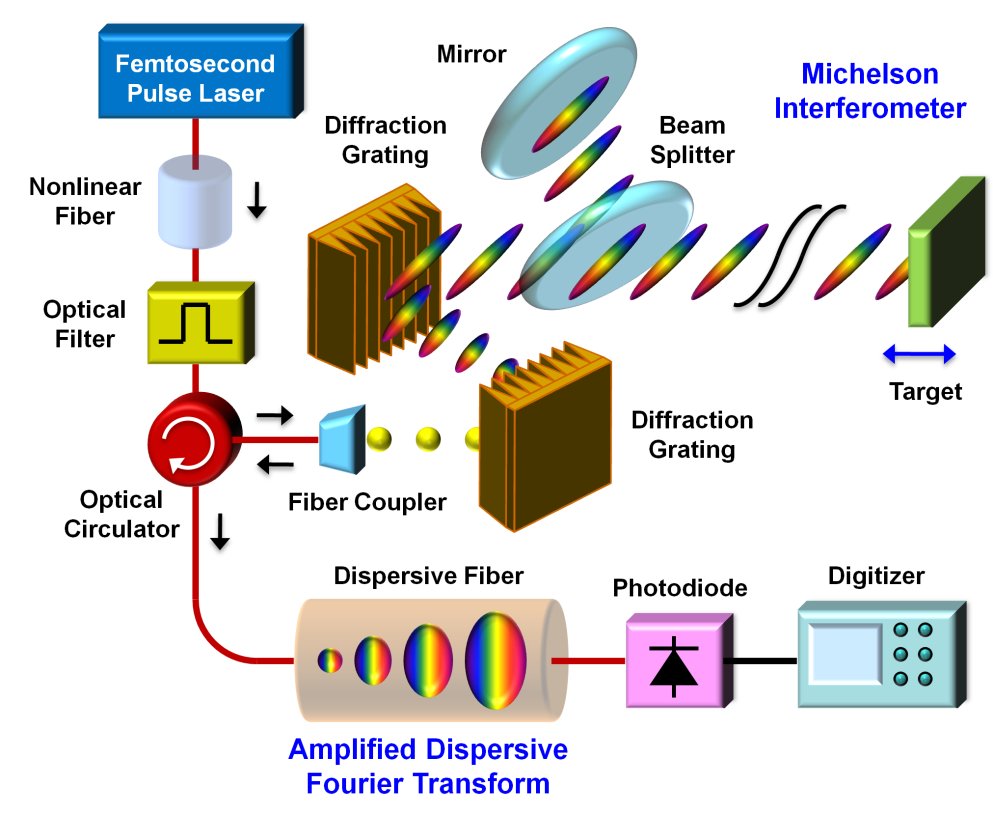
\includegraphics[scale=1]{APL2011/Figure1.png}
\caption{Schematic of the STEAM vibrometer. The principle of the method is three-fold: (1) encoding of the lateral and axial coordinates of the target into the different frequencies and corresponding amplitudes of a spatially dispersed broadband pulse which spectrally interferes with a reference pulse, (2) amplified dispersive Fourier transformation in which the spectrum is mapped into a temporal waveform, time-stretched so that it can be digitized in real time, and simultaneously amplified in the optical domain, and (3) Hilbert transformation on the detected pulse in the digital domain to extract the axial information of the target.}
\label{fig:APL2011_Figure1}
\end{figure}

The interferometrically combined pulses return to the same optics, but are directed via an optical circulator toward the amplified dispersive Fourier transformer (ADFT) \cite{goda2009serial, goda2008amplified, goda2009theory} in which a dispersive fiber with -1200 ps/nm dispersion is optically pumped by four continuous-wave lasers with $\sim$100 mW of optical power at 1470 nm, 1480 nm, 1480 nm, and 1490 nm for distributed Raman amplification. In the dispersive medium, the spectrum of each interfered pulse is stretched and converted into an amplified temporal waveform. This ADFT process is critical for high-speed laser vibrometry because the optical amplification before photon-to-electron conversion overcomes the fundamental trade-off between sensitivity and speed \cite{goda2009serial, goda2009theory}. The pulses are captured by a high-speed photodiode with 15 GHz bandwidth and digitized by a real-time oscilloscope with 16 GHz bandwidth and 50 GS/s sampling rate. Hilbert transformation is applied in the digital domain to each spectrally interfered pulse to obtain the axial information of the target at multiple points along the 1D line. Each pulse acquires one scan and the pulse repetition rate corresponds to the scan rate (frame rate) of the STEAM vibrometer.

\section{Theoretical study of the vibrometer performance}

The basic capabilities of the STEAM vibrometer (i.e., image pixel number, axial resolution, and dwell time) can be estimated from the parameters of its components. First, the number of image pixels on the target ($ N $) is found from the total dispersion in the dispersive fiber ($ D = \SI{-1200}{ps/nm} $), the optical bandwidth ($ \Delta\lambda = \SI{20}{nm} $), and the sampling rate of the digitizer ($ f_{dig} = \SI{50}{GS/s} $) to be $ N = |D| \cdot \Delta\lambda \cdot f_{dig} = 1200 $ while the number of resolvable points is about 200 from the spectral resolution of the ADFT process [16]. Second, the axial resolution is given by the dynamic range (bit depth) of the digitizer. The axial resolution ($\Delta z$) can be found from the expression, $0.5 \sin(2 \cdot k \cdot \Delta z) = 2^{-n}$, where $k$ is the wavenumber [$k = 2 \pi / (\SI{1590}{nm})$] and $n$ is the bit depth of the digitizer ($n = \SI{8}{bits}$), to be $\Delta z = \SI{0.99}{nm}$. Finally, the dwell time is estimated from the bandwidth of each subpulse ($\SI{20}{nm} /$$\sim$$\num{200}$) and the time-bandwidth product to be $\sim$\SI{30}{ps} (assuming that the subpulses are transform limited).

\section{Experimental results}

We evaluated the basic performance of the STEAM vibrometer. In Figure \ref{fig:APL2011_Figure2}a, the temporal waveform of a single interfered pulse captured by the photodiode is compared with the optical spectrum measured by a conventional optical spectrum analyzer. This verifies the equivalence of the two waveforms and hence validates the STEAM vibrometer. As shown in Figure \ref{fig:APL2011_Figure2}b, repetitive pulses (scans) detected by the photodiode indicate that the STEAM vibrometer operates at 36.7 MHz scan rate.

\begin{figure}[htb!]
\centering
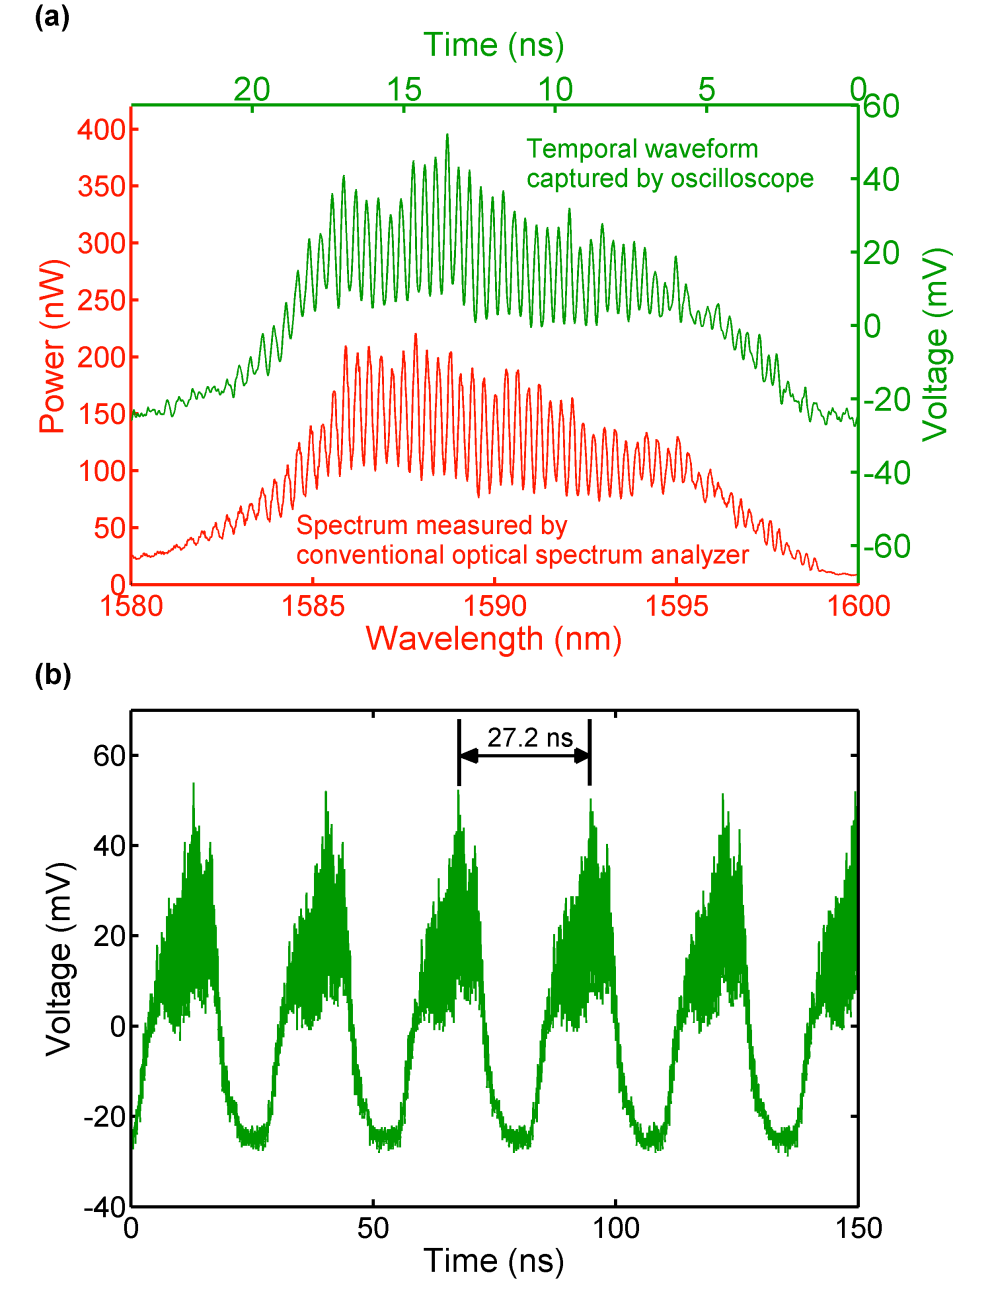
\includegraphics[scale=1]{APL2011/Figure2.png}
\caption{Basic performance of the STEAM vibrometer. (a) Temporal waveform of a single interfered pulse captured by the photodiode in comparison with the optical spectrum measured by a conventional optical spectrum analyzer. (b) Repetitive pulses (scans) with a time interval of 27.2 ns detected by the photodiode indicating that the STEAM vibrometer operates at 36.7 MHz scan rate.}
\label{fig:APL2011_Figure2}
\end{figure}

To show the utility of the STEAM vibrometer, we monitored the performance of an acoustic speaker. For better sensitivity, a thin reflective plate was attached to the diaphragm of the acoustic speaker. The speaker was driven up to 30 kHz (nearly its upper frequency limit). Figure \ref{fig:APL2011_Figure3} shows the 30 kHz surface vibration of the diaphragm captured by the STEAM vibrometer with $\sim$1 nm axial resolution (which agrees with our estimated axial resolution of 0.99 nm).

\begin{figure}[htb!]
\centering
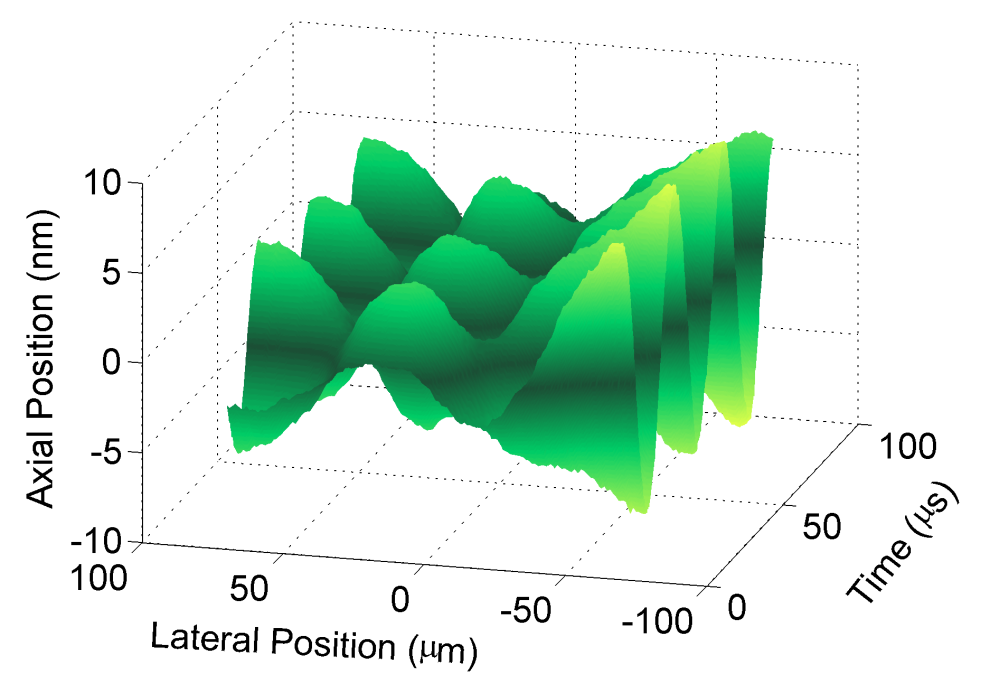
\includegraphics[scale=1]{APL2011/Figure3.png}
\caption{Surface vibration of the acoustic diaphragm captured by the STEAM vibrometer with $\sim$1 nm axial resolution and $\sim$30 ps dwell time. The diaphragm was driven to vibrate at 30 kHz.}
\label{fig:APL2011_Figure3}
\end{figure}

In addition to the amplitude of the surface vibration, we also obtained the velocity of the diaphragm from the axial coordinates of the surface as shown in Figure \ref{fig:APL2011_Figure4}. The Doppler frequency shift in the frequency comb lines caused by the acoustic vibration ($\sim$830 Hz frequency shift) is negligible.

\begin{figure}[htb!]
\centering
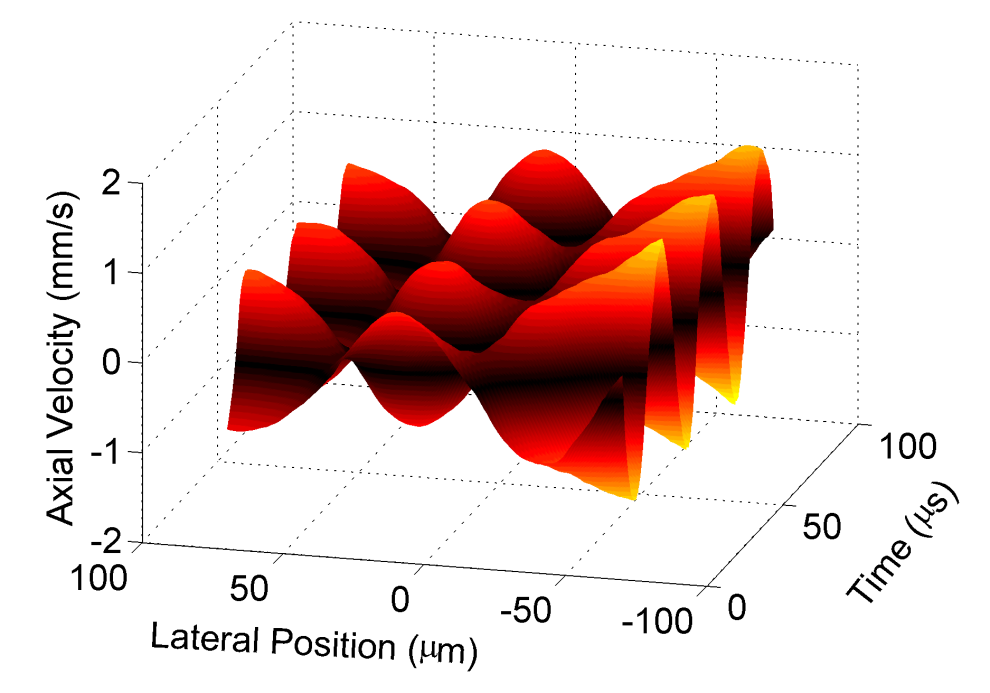
\includegraphics[scale=1]{APL2011/Figure4.png}
\caption{Axial velocity of the acoustic diaphragm obtained by the STEAM vibrometer. The diaphragm was driven to vibrate at 30 kHz (the same as in Figure \ref{fig:APL2011_Figure3}).}
\label{fig:APL2011_Figure4}
\end{figure}

\section{Conclusion}

In summary, we proposed and demonstrated an optical system that performs high-speed multi-dimensional imaging-based vibrometry and velocimetry with nanometer-scale axial resolution without the need for beam scanning. As a proof-of-concept, we showed real-time 1D imaging of fast acoustic vibrations with 1 nm axial resolution, 1200 image pixels, and 30 ps dwell time at 36.7 MHz scan rate. While we performed 1D cross-sectional imaging in this proof-of-principle demonstration, the technique can naturally be extended to 2D by using a 2D spatial disperser \cite{goda2009serial,tsia2010performance}.

                         % Chapter 2
\chapter{3D Ultrafast Laser Scanner}

Laser scanners are essential for scientific research, manufacturing, defense, and medical practice. Unfortunately, often times the speed of conventional laser scanners (e.g., galvanometric mirrors and acousto-optic deflectors) falls short for many applications, resulting in motion blur and failure to capture fast transient information. Here, we present a novel type of laser scanner that offers roughly three orders of magnitude higher scan rates than conventional methods. Our laser scanner, which we refer to as the hybrid dispersion laser scanner, performs inertia-free laser scanning by dispersing a train of broadband pulses both temporally and spatially. More specifically, each broadband pulse is temporally processed by time stretch dispersive Fourier transform and further dispersed into space by one or more diffractive elements such as prisms and gratings. As a proof-of-principle demonstration, we perform 1D line scans at a record high scan rate of 91 MHz and 2D raster scans and 3D volumetric scans at an unprecedented scan rate of 105 kHz. The method holds promise for a broad range of scientific, industrial, and biomedical applications. To show the utility of our method, we demonstrate imaging, nanometer-resolved surface vibrometry, and high-precision flow cytometry with real-time throughput that conventional laser scanners cannot offer due to their low scan rates.

\section{Introduction}

High-speed multidimensional laser scanning technology has numerous applications in research \cite{marshall2011handbook,fujii2005laser,dotson2003fundamentals,popescu2006optical,gobel2006imaging,pawley2010handbook,denk1990two,wandinger2005lidar}, manufacturing \cite{marshall2011handbook,fujii2005laser,dotson2003fundamentals,schwarz2010mapping,sinha2010vibration,pelesko2002modeling,osten2006optical,horn1986robot}, defense \cite{marshall2011handbook,fujii2005laser,schwarz2010mapping,sinha2010vibration,horn1986robot}, and biomedicine\cite{marshall2011handbook, popescu2006optical,gobel2006imaging,pawley2010handbook,denk1990two,hoffman2006confocal,tarnok2002clinical,vacca2009laser} for sensing and imaging of moving objects and dynamic processes. Low scan rates cause motion blur in images or missing fast transient phenomena in sensing. Also, high-speed scanning capability is needed in high-throughput analysis of a large number of objects or a wide field of view in a reasonable duration of time \cite{marshall2011handbook,fujii2005laser,dotson2003fundamentals,wandinger2005lidar,horn1986robot,hoffman2006confocal,tarnok2002clinical,vacca2009laser,mahjoubfar2011high}.

Various types of laser scanners have been developed over the past few decades. The most commonly used type of laser scanners including MEMS scanners \cite{conant2002micromachined} is based on beam steering by galvanometric mirrors. However, their linear scan rates because of inertia are limited to about 10 kHz. If two of these scanners are aggregated to perform 2-dimensional (2D) raster scans, the overall raster scan rate is limited to about 100 Hz. Another type of laser scanner is based on diverting laser beams by acousto-optic deflectors (AODs). They are about one order of magnitude faster than galvanometric mirror scanners in both linear and 2D raster scans \cite{marshall2011handbook,pape1994design}. Finally, a combination of a frequency-tunable laser and diffractive optics can be used to form a laser scanner at scan rates comparable to AODs \cite{yaqoob2004passive,boudoux2005rapid}.

Recently, we have demonstrated a new type of inertia-free ultra-fast laser scanner that can achieve about three orders of magnitude faster scan rates than the conventional methods \cite{goda2012hybrid}. The operation principle of this method, namely the hybrid dispersion laser scanner (HDLS), is based on probing different points of a target with frequency components of a linearly chirped broadband optical pulse at different times. In this chapter, we present results from our demonstration of linear scans at 90.8 MHz, 2D raster scans at 105.4 kHz, and 3D scanning surface vibrometry with nanometer axial resolution.

\section{Principle of Hybrid dispersion laser scanner}

The concept of HDLS relies on the transformation from spectral to temporal and spatial domains, respectively (Figure \ref{fig:PW2013_Figure1}). First, by a process called dispersive Fourier transformation \cite{kelkar1999time,chou2007femtosecond,goda2009theory,goda2009serial,goda2008amplified} based on group-velocity dispersion, the spectra of broadband optical pulses of a mode-locked laser are mapped into temporal waveforms. Then, a spatial dispersive element such as a diffraction grating or a virtually imaged phased array (VIPA) maps the spectrum of chirped pulses onto a line over the object such that different wavelength components hit the target at different positions and times. The reflected or scattered light from the target is then detected by a single-pixel photodetector. Wavelength components of each laser pulse perform one linear scan, and therefore, the scan rate is same as the repetition rate of the mode-locked laser. A complementary scanner for other axis can be added to achieve 2D raster scans with HDLS.

\begin{figure}[htb!]
\centering
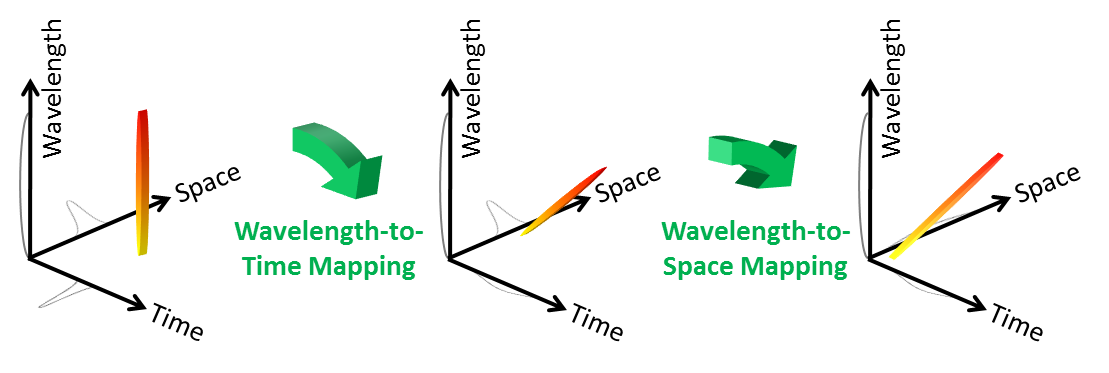
\includegraphics[scale=0.65]{PW2013/Figure1.png}
\caption{Concept of HDLS. HDLS operation relies on two high-speed mapping processes. First, the spectrum of each broadband optical pulse generated by a mode-locked laser is mapped to time. This wavelength-to-time mapping is performed by a temporal dispersive element such as a dispersive optical fiber or prism pair. Next, wavelength-to-space transformation is used to direct each wavelength component of the optical pulse to a unique point on the target. Overall, a one-to-one mapping between time and space is formed. Therefore, each point in HDLS’ field of view is sampled with an individual wavelength component of the optical pulse at a specific time. The repetition rate of the mode-locked laser determines the sampling rate of the HDLS.}
\label{fig:PW2013_Figure1}
\end{figure}

Based on the HDLS concept described, we designed and implemented a multi-dimensional laser scanner in the industrially and biomedically important spectral range of 800 nm (Figure \ref{fig:PW2013_Figure2}). A Ti:Sapphire femtosecond mode-locked laser with a repetition rate of 90.8 MHz generates a train of broadband optical pulses centered at 814 nm. The process of wavelength-to-time mapping is performed with two pairs of prisms followed by a dispersive fiber. Pulses are then collimated into free space and scanned in the vertical direction by an acousto-optic deflector at 105.4 kHz. A pair of diffraction gratings performs the wavelength-to-space mapping, which is the key to fast scanning capability of HDLS at 90.8 MHz in the horizontal direction. 

Different wavelength components of each laser pulse hit the target at different times, such that a single-pixel photodetector can be used to measure their reflections. The electrical signal of the photodetector corresponding to the waveform of the reflected optical pulses is captured by a high-speed digitizer (50 GS/s, 20 GHz bandwidth oscilloscope) (Figure \ref{fig:PW2013_Figure3}a). Digital waveforms are processed and combined in Matlab to generate multi-dimensional scan profiles. To validate the wavelength-to-time mapping implemented by the prism pairs and dispersive fiber, the spectrum of the reflected pulses from a fixed target is measured with a conventional spectrum analyzer and compared to the waveforms captured by the oscilloscope (Figure \ref{fig:PW2013_Figure3}b). Good agreement between them confirms that we can measure the spectral information of laser pulses at the pulse repetition rate of the mode-locked laser that is well beyond the scan rate of conventional spectrum analyzers.

\section{Applications of Hybrid dispersion laser scanner}

In order to visualize the operation of the HDLS, we scanned a high-reflective substrate with letters “UCLA” engraved on it, and compared the results side-by-side with an image taken by a regular CCD camera (Figure \ref{fig:PW2013_Figure4}). For this experiment, the target was 90 degrees rotated around the illumination axis with respect to the images shown, so that the vertical scans in the image are performed by the HDLS while horizontal scans in the image are implemented by the AOD.

\begin{figure}[htb!]
\centering
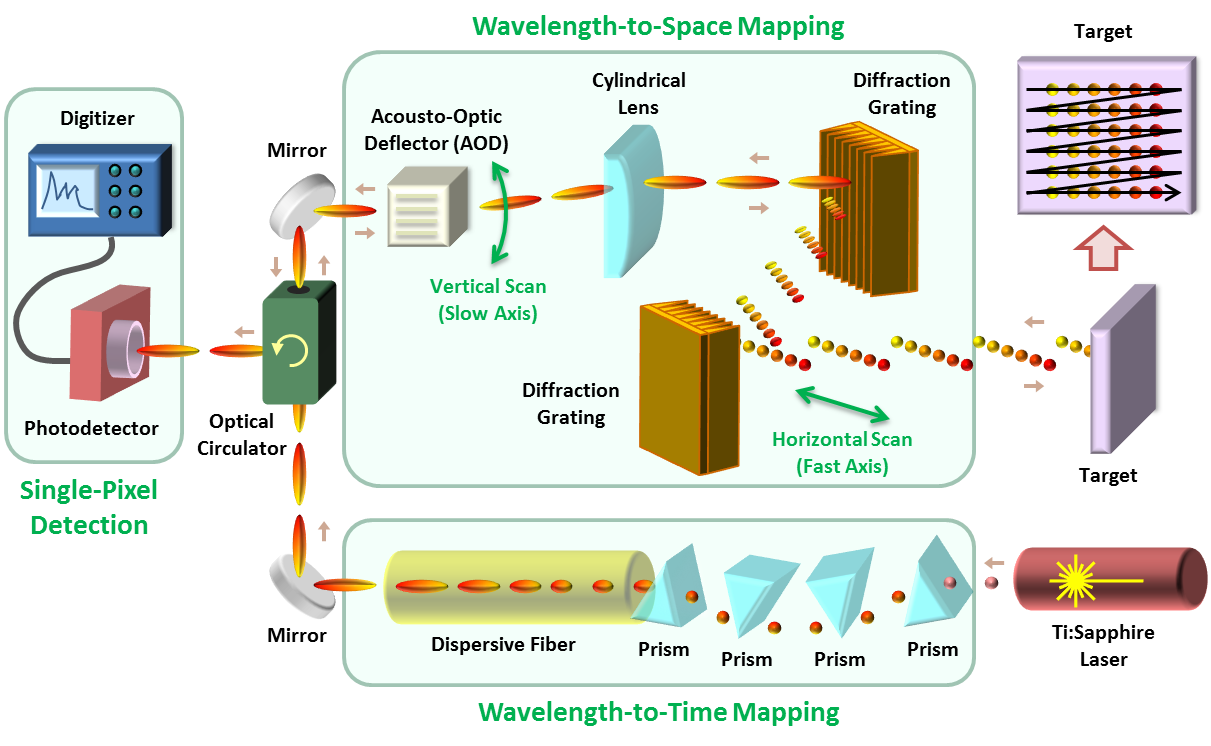
\includegraphics[scale=0.65]{PW2013/Figure2.png}
\caption{HDLS experimental setup. In a 2D demonstration of laser scanning with the HDLS, optical pulses generated by a mode-locked Ti:Sapphire laser with a center wavelength of 814 nm and a repetition rate of 90.8 MHz are dispersed in time using two pairs of prisms and a dispersive fiber. Pulses are deflected in the vertical direction using an acousto-optic deflector (AOD) at 105.4 kHz. Subsequently, the spectrum of each pulse is mapped onto a horizontal line using a pair of diffraction gratings. A combination of the vertical deflection and horizontal mapping leads to a 2D raster scan on the target. The pulse reflection off the surface of the target is converted via an optical circulator to an electrical signal using a single-pixel high-speed photodetector. This is possible due to the prior wavelength-to-time mapping, so that each wavelength component reaches the photodetector at a unique time, and the information of different points of the target are not overlapped. A 50 GS/s digitizer acquires the electrical signal from the photodetector, which corresponds to the spectrum of the optical pulses. After correction for the background envelope, the spectrum of each pulse reveals one horizontal line scan image of the target. Stacking up many of these line scans in accordance with the AOD scan frequency leads to a 2D raster scan of the target.}
\label{fig:PW2013_Figure2}
\end{figure}


\begin{figure}[htb!]
\centering
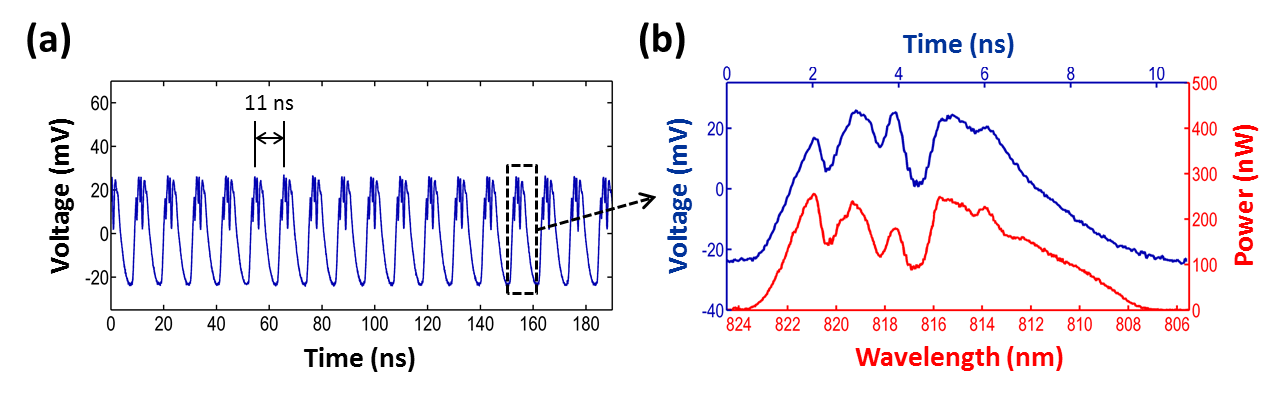
\includegraphics[scale=0.65]{PW2013/Figure3.png}
\caption{Wavelength-to-time mapping with dispersive Fourier transformation. (a) Optical pulses reflected off the target corresponding to horizontal line scans at different deflection angles of the AOD are measured by a high-speed photodetector. The period of the horizontal scans is about 11 ns, which corresponds to the mode-locked laser’s pulse repetition rate (90.8 MHz). (b) Good agreement between the amplitude of the photodetector signal measured with the digitizer (shown in blue) and the power spectrum measured with a conventional optical spectrum analyzer indicates the demonstration of the wavelength-to-time mapping using the prism pairs and dispersive fiber in the 800 nm band.}
\label{fig:PW2013_Figure3}
\end{figure}

\begin{figure}[htb!]
\centering
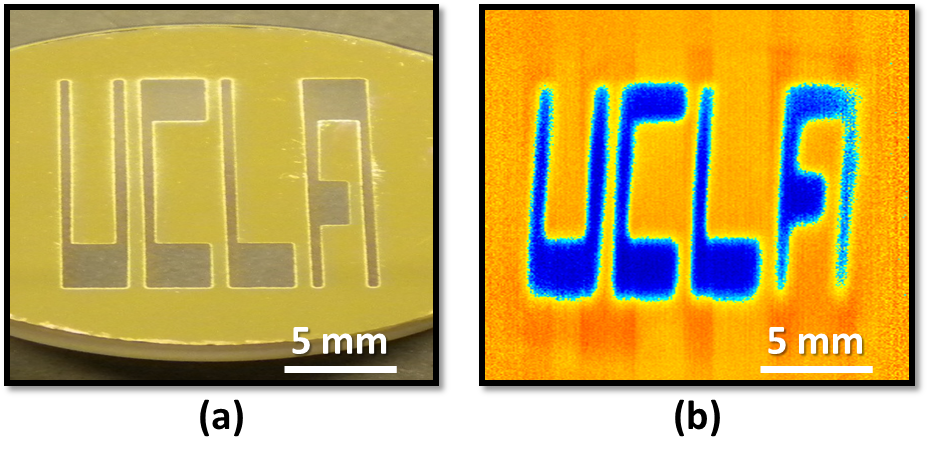
\includegraphics[scale=0.9]{PW2013/Figure4.png}
\caption{Imaging with the HDLS. (a) Image of the word “UCLA” engraved on the surface of a reflective substrate captured by a CCD camera. (b) Image of the same sample captured by the HDLS. The word “UCLA” is clearly shown. 
Combining the HDLS with an interferometer, we performed 3D surface profilometry or 2D surface vibrometry (Figure \ref{fig:PW2013_Figure5}). Here we used a Michelson interferometer to encode phase delays of different points on the target into wavelength components of the illumination pulses. The interferograms are then captured in time, and analyzed offline by Hilbert transformation to extract the phase variations, which correspond to the axial positions. Our experimental setup enables an axial resolution of 0.4 nm at a scan rate of 105.4 kHz. As an illustrative demonstration, we captured vibrations of a reflective diaphragm oscillating at 1 kHz (Figure \ref{fig:PW2013_Figure6}).}
\label{fig:PW2013_Figure4}
\end{figure}
 
\begin{figure}[htb!]
\centering
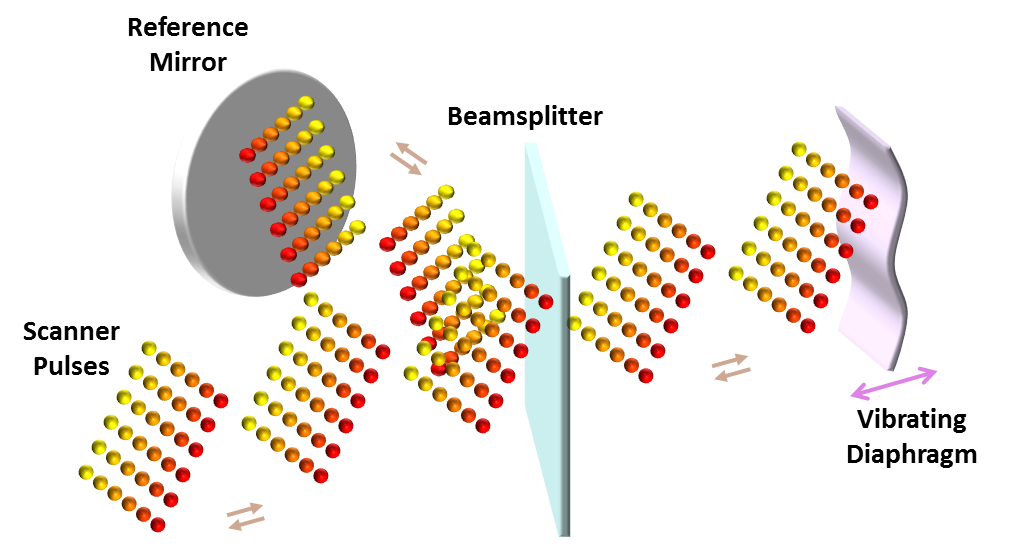
\includegraphics[scale=0.85]{PW2013/Figure5.png}
\caption{3D surface profilometry or 2D surface vibrometry with the HDLS. 2D raster scans by the HDLS are used in conjunction with a Michelson interferometer to perform 2D surface vibrometry. A beamsplitter splits scan pulses into two arms. Optical pulses in one arm hit the target, and the light in the other arm (reference arm) is reflected intactly by a mirror. Reflected pulses from both arms are combined at the beamsplitter and form an interference pattern. If the reflectivity of the vibrating target is not changing rapidly, Hilbert transformation can be used to extract the relative optical phase of each wavelength component. Therefore, variations of the optical path length at each wavelength component are measured and used to form 3D surface profiles of the vibrating sample at a scan rate of 105.4 kHz with 0.4 nanometer axial resolution.}
\label{fig:PW2013_Figure5}
\end{figure}
 
\begin{figure}[htb!]
\centering
\includegraphics[scale=0.68]{PW2013/Figure6.png}
\caption{Surface vibration captured by the HDLS. Frames from 3D scans of a vibrating diaphragm by the HDLS show a period of nanomechanical vibrations at 1 kHz. Only one every ten scan is shown here.}
\label{fig:PW2013_Figure6}
\end{figure}

Finally, as an example of the HDLS’ biomedical utility, we demonstrated high-precision high-throughput flow cytometry using the HDLS. Low spatial resolution of conventional flow cytometers causes a considerable number of false positive events that result in statistical error in subpopulation analysis. For instance, they are not effective for detection of multiple cells (i.e., doublets, triplets, etc.) (Figure \ref{fig:PW2013_Figure7}a). We used inertial focusing microfluidic technology \cite{di2009inertial} to precisely align otherwise randomly positioned cells in a single stream with no need for sheath flow (Figure \ref{fig:PW2013_Figure7}b). The microfluidic channel is custom-made on a substrate dielectric mirror from thermoset polyester (TPE) for stability, robustness, and increased precision of cell focusing. HDLS pulses scan the stream of cells, and the forward scattering is reflected back by the substrate mirror for measurement. 

We tested the performance of the HDLS and conventional flow cytometer for size-based identification of white blood cells and MCF7 breast cancer cells (Figure \ref{fig:PW2013_Figure7}c). Since the HDLS flow cytometer is more precise in distinguishing multiple cells e.g. doublets, the count of white blood cells that have unusually larger size is reduced, and therefore, the false positive rate decreases. This improvement in size-based classification of MCF7 breast cancer cells from white blood cells is more evident in comparison of receiver operating characteristic (ROC) curves of the HDLS and conventional flow cytometer (figure 2-7d). We observed that for the same specificity, the sensitivity of our method is significantly higher than that of the conventional flow cytometer. 
 
\begin{figure}[htb!]
\centering
\includegraphics[scale=0.65]{PW2013/Figure7.png}
\caption{Comparison of conventional and HDLS flow cytometers. (a) In regular flow cytometry, a single interrogation beam covers the desired field of view in the channel. Therefore, it does not efficiently differentiate multiple cells such as doublets. In HDLS flow-cytometer, diffraction limited wavelength components of the interrogation beam cover the required field of view, and extract high-resolution spatial information of the sample. HDLS data can be used to identify abnormalities e.g. multiple cells and result in a lower statistical error. (b) In our demonstration of HDLS flow cytometer, an inertial focusing microfluidic channel with a dielectric mirror substrate is used to order randomly distributed cells into a single stream. The microfluidic device was fabricated using standard replica molding methods in thermoset polyester (TPE) to ensure stability. HDLS scan pulses are focused on the stream. Forward-scattered light from the cells is reflected by substrate mirror and collected by an objective lens. (c) Identical samples of white blood cells and MCF7 breast cancer cells are measured separately with conventional and HDLS flow cytometers. There is a considerable overlap in forward scattering range of these cell types for a conventional flow cytometer. However, this overlap decreases significantly for HDLS flow cytometer measurements because white blood cell multiples are not identified as MCF7 cancer cells. (d) Receiver operating characteristic (ROC) curves based on identification of white blood cells and MCF7 breast cancer cells show that without sacrificing throughput, HDLS flow cytometer achieves higher specificity and sensitivity than a conventional flow cytometer.}
\label{fig:PW2013_Figure7}
\end{figure}
                         % etc.
\chapter{Label-free high-throughput cell screening}
\label{chp:BOE2013_Chapter}

Flow cytometry is a powerful tool for cell counting and biomarker detection in biotechnology and medicine especially with regards to blood analysis. Standard flow cytometers perform cell type classification both by estimating size and granularity of cells using forward- and side-scattered light signals and through the collection of emission spectra of fluorescently-labeled cells. However, cell surface labeling as a means of marking cells is often undesirable as many reagents negatively impact cellular viability or provide activating/inhibitory signals, which can alter the behavior of the desired cellular subtypes for downstream applications or analysis. To eliminate the need for labeling, we introduce a label-free imaging-based flow cytometer that measures size and cell protein concentration simultaneously either as a stand-alone instrument or as an add-on to conventional flow cytometers. Cell protein concentration adds a parameter to cell classification, which improves the specificity and sensitivity of flow cytometers without the requirement of cell labeling. This system uses coherent dispersive Fourier transform to perform phase imaging at flow speeds as high as a few meters per second.

\section{Introduction}

Cell protein content measurement can be used in many biomedical applications such as blood doping detection \cite{grover2011measuring}, infection monitoring \cite{mrema1979concentration}, drug development and screening \cite{chun2012rapidly}, studies of necrosis and apoptosis \cite{martin1990hl,wyllie1982hormone}, cell cycle progression and differentiation \cite{wolff1972separation,maric1998buoyant,bista2011quantification}, and in cancer diagnostics \cite{bosslet1981rapid,phillips2012quantification,phillips2012optical}. Current methods for cell protein concentration measurement include electrical methods based on dielectrophoresis \cite{gupta2012apostream}, mechanical methods based on microchannel cantilevers \cite{grover2011measuring}, and optical methods based on scattering patterns \cite{tycko1985flow}, emission spectra of external cavity lasers \cite{liang2007determining}, and holographic and phase microscopy \cite{rappaz2005measurement,curl2005refractive,lue2009live,gorthi2012phase}. These methods are either inherently too slow for high-speed flow cytometry applications or require feedback mechanisms \cite{popescu2006optical} to provide necessary precision. Furthermore, size-based classification can also be used for label-free identification of cells of interest in a suspension stream \cite{vona2000isolation}. However, due to significant overlap of size ranges between most mammalian cells, size-based technologies require additional layers of parametric gating to be useful as a diagnostic tool \cite{di2013hyperspectral}.  It is known that the refractive index of a cell is proportional to its protein content \cite{barer1954refractometry}. As such, the simultaneous measurement of refractive index and size of cells would be predicted to provide two independent parameters for cell classification.

In this chapter, we propose a fast and high-precision optical cell density and size measurement method based on serial time-encoded amplified microscopy (STEAM) \cite{goda2009serial}. STEAM is a continuous imaging technique that captures tens of million frames-per-second with sub-nanosecond shutter speed. However, earlier versions of STEAM were dependent on cell labeling due to low intensity contrast of individual cells \cite{goda2012high}. Here, we introduce a new configuration of STEAM capable of high-speed phase microscopy and demonstrating label-free single-cell classification and diagnostics. In addition, we demonstrate a new design of STEAM that minimizes loss and chromatic aberration, decreases polarization sensitivity, and results in a smaller footprint \cite{fard2011nomarski}. In contrast to previous implementations of STEAM, which were based on refractive optics, the new design employs reflective optics.

The basic principle of STEAM involves two steps both performed optically. In the first step, the spectrum of a broadband optical pulse is converted by a spatial disperser into a rainbow that illuminates the target. Therefore, the spatial information (image) of the object is encoded into the spectrum of the resultant reflected or transmitted rainbow pulse. A 1D rainbow is used in flow imaging as the flow causes the cell to be scanned in the second dimension. In the second step, the spectrum of the image-encoded pulse is mapped into a serial temporal signal that is stretched in time to slow it down such that it can be digitized in real-time \cite{goda2013dispersive}. This optically-amplified time-stretched serial stream is detected by a single-pixel photodetector and the image is reconstructed in the digital domain. Subsequent pulses capture repetitive frames, hence the laser pulse repetition rate corresponds to the frame rate of STEAM and the shutter speed (exposure time) corresponds to the temporal width of the pulse. The key innovations in STEAM that enable high speed real-time imaging are photonic time stretch for digitizing fast images in real-time and the optical image amplification for compensating the low number of photons collected during the ultra-short shutter time.

The contrast limitations of label-free single-cell imaging of STEAM led us to develop a derivative of STEAM, referred to as Coherent-STEAM, to capture phase images of cells in flow. We use a Michelson interferometer to map the phase image of cells into the spectrum of broadband optical pulses. This phase imaging technique exploits the fast shutter speed of STEAM to freeze path length fluctuations of interferometer arms and attains nanometer phase resolution with no need for feedback stabilization of the interferometer \cite{mahjoubfar2011high,goda2012hybrid,mahjoubfar20133d}. We use Coherent-STEAM to measure the refractive index of individual cells in an imaging flow cytometer by simultaneous measurement of size and total optical phase-shift induced by the cells. As an example, we use our label-free STEAM-based cell classifier to distinguish OT-II T cell hybridoma from SW480 epithelium cancer cells. We show that adding protein concentration to size as an additional classification parameter increases accuracy and specificity in flow cytometry.

\section{Experimental setup}

A mode-locked fiber laser generates pulses at 1565 nm with a repetition rate of 36.128 MHz and a pulse width slightly less than 100 fs (Figure Figure \ref{fig:BOE2013_Figure1}). Pulses are spectrally broadened with a highly nonlinear fiber to approximately 100 nm bandwidth \cite{boyraz2000broadband}. A short dispersion compensating fiber with an overall dispersion of 60 ps/nm is used to temporally broaden pulses to 1.2 ns, so an erbium doped fiber amplifier (EDFA) can amplify them without any distortion. Amplified pulses enter a coarse wavelength division multiplexing (WDM) filter, and the output of 1591 nm channel is used to shape laser pulses with a considerably flat spectrum over 1581 nm to 1601 nm bandwidth. These pulses pass through an optical circulator and are coupled to free-space with a fiber collimator.

\begin{figure}[htb!]
\centering
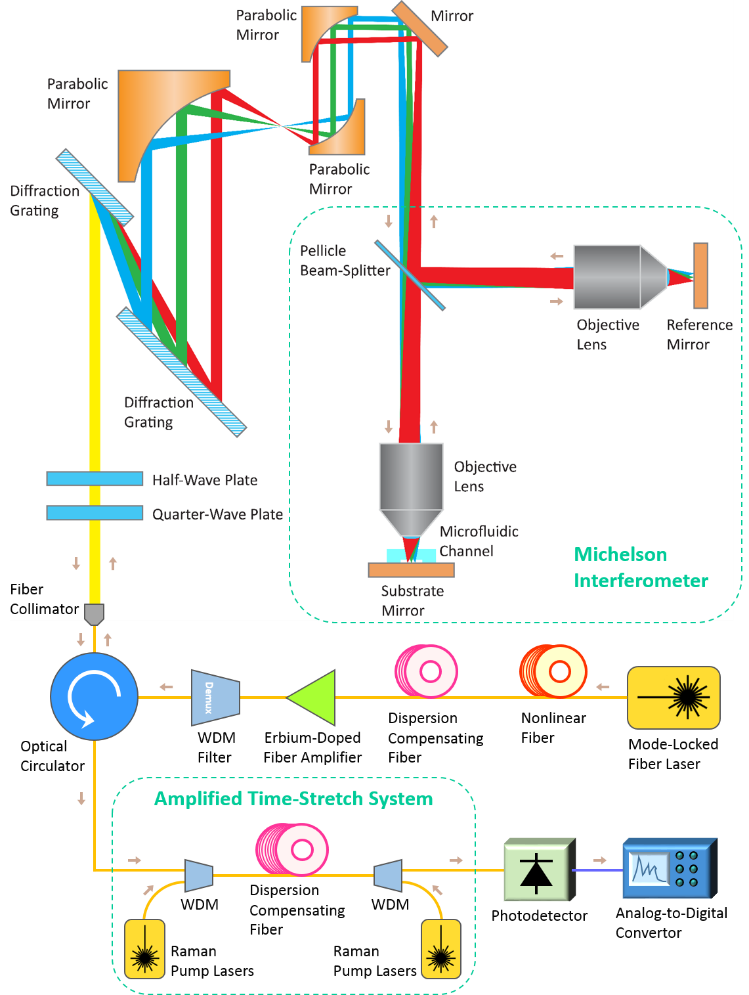
\includegraphics[scale=1]{BOE2013/Figure1.png}
\caption{Optical setup of Coherent-STEAM. A Coherent-STEAM setup is formed by combination of STEAM and a Michelson interferometer. A pair of diffraction gratings generates a 1D rainbow with different wavelength components imaging different points on the cells flowing in a microfluidic channel. A pellicle beam-splitter and two identical long working-distance objective lenses are used to form the interferometer for phase measurement. Back apertures of objective lenses are fully illuminated with each wavelength component of the broadband mode-locked laser pulses to ensure diffraction-limited resolution. An amplified time-stretch system chirps, stretches, and amplifies each pulse, so that different wavelength components reach the photodetector serially. A very shallow microfluidic channel with hydrodynamic focusing is designed and fabricated to align cells within the focal depth of the system.}
\label{fig:BOE2013_Figure1}
\end{figure}

Free-space laser pulses are linearly polarized with quarter- and half-wave plates, and then they are spatially dispersed with a pair of reflection diffraction gratings, so that each wavelength component of the collimated beam is positioned at a different lateral point similar to a rainbow. A pair of 90 degree off-axis parabolic gold-coated mirrors with 152.4 mm and 25.4 mm reflected focal lengths are used to form a beam reducer that shrinks the rainbow beam 6 times. Parabolic gold-coated mirrors are used to minimize loss, aberration, and polarization sensitivity. In addition, a 15 degree off-axis parabolic gold-coated mirror with 635 mm reflected focal length and a 0.4 numerical aperture long working-distance objective lens further shrink the rainbow to about 130 $\mathrm{\mu}$m field of view. Using reflective optics, we managed to improve the signal-to-noise ratio by about 9 dB. A beam splitter is used to form two arms of a Michelson interferometer. Different wavelength components of the rainbow are focused on a mirror in the reference arm and on the reflective substrate of a microfluidic device in the sample arm. Cells hydrodynamically focused at the center of the channel flow at a velocity of 1.3 m/s. The rainbow pulses pass through the cells and are reflected back by the mirror substrate of the microfluidic device. The total bandwidth of the pulses interrogating the cells in our Coherent STEAM is less than 20 nm centered at 1590 nm, giving a negligible fractional bandwidth of 1.3\%. Therefore, the color-dependency of absorption is very small and can be easily neglected. The reflected pulses from the microfluidic device and reference mirror interfere at the beam splitter and return to the fiber, where they are directed with the optical circulator to an amplified time-stretch system.

The amplified time-stretch system is a combination of a Raman amplifier and a dispersive fiber to perform dispersive Fourier transform \cite{goda2013dispersive}. Four Raman pump lasers at 1450 nm, 1470 nm, 1490 nm, and 1505 nm are used to amplify the signal for about 15 dB over the whole optical bandwidth uniformly. The dispersive fiber chirps and stretches each pulse in time to about 27 ns. So, different wavelength components reach the photodetector serially. An analog-to-digital converter (ADC) with a sampling rate of 50 GSps and 20 GHz bandwidth is used to acquire the output signal of the photodetector.

The photodetector output signal, $I(t)$, is digitized and recorded by the ADC (Figure \ref{fig:BOE2013_Figure2}a). This signal shows sequential laser pulses. Each pulse is used to form one line image. Therefore, the boundaries of pulses are determined precisely, and each pulse is saved separately as a frame for further processing (Figure \ref{fig:BOE2013_Figure2}b). The analytic form of each pulse is generated using Hilbert transformation after the low frequency components corresponding to intensity variations are filtered out \cite{ikeda2005hilbert}. The phase component of this analytic form is extracted, while its amplitude component is discarded (Figure \ref{fig:BOE2013_Figure2}c). Because the phase varies over a wide range (much larger than $2 \pi$ radians), it shows unrealistic discontinuities. An unwrapping algorithm is used to fix these discontinuities, and the result shows an approximately linear phase increase over the time for each pulse or frame (Figure \ref{fig:BOE2013_Figure2}d). The unwrapping algorithm adds multiples of $\pm 2 \pi$ to make the absolute jumps between consecutive samples in a frame smaller than $\pi$ radians when they are greater than $\pi$ radians. If the linear component of the phase, which corresponds to the fringe (modulation) frequency, $f_m$, due to the interferometer arms' length mismatch, and the background phase level, $\varphi_0$, are subtracted, the phase shift induced by the cells in the optical pulse can be observed (Figure \ref{fig:BOE2013_Figure2}e); i.e. 
\begin{equation}
\Delta\varphi(t)= unwrap(\arg(I_{BP}(t)+j \cdot \hat{I}_{BP}(t))) - 2 \pi f_m t - \varphi_0
\end{equation}
in which $I_{BP}(t)$ is a band-pass filtered form of $I(t)$ with only spectral features modulated at $f_m$, and $\hat{I}_{BP}(t)$ is the Hilbert transform of $I_{BP}(t)$. Many phase line images generated from subsequent frames are combined to form a spatial map of optical path difference (OPD) in two dimensions (Figure \ref{fig:BOE2013_Figure2}f). Since we know the mapping of space to time from the rainbow characteristics and flow speed, OPD at each point is calculated as
\begin{equation}
OPD(x,y) = \frac{\lambda(x)}{2 \pi} \Delta\varphi(x,y)
\end{equation}
where $x$ and $y$ are coordinates in the rainbow and flow directions, respectively; $\lambda(x)$ is the wavelength at position $x$ along the rainbow; and $\Delta\varphi(x,y)$ is the phase shift induced by the cell at point $(x,y)$.

\begin{figure}[htb!]
\centering
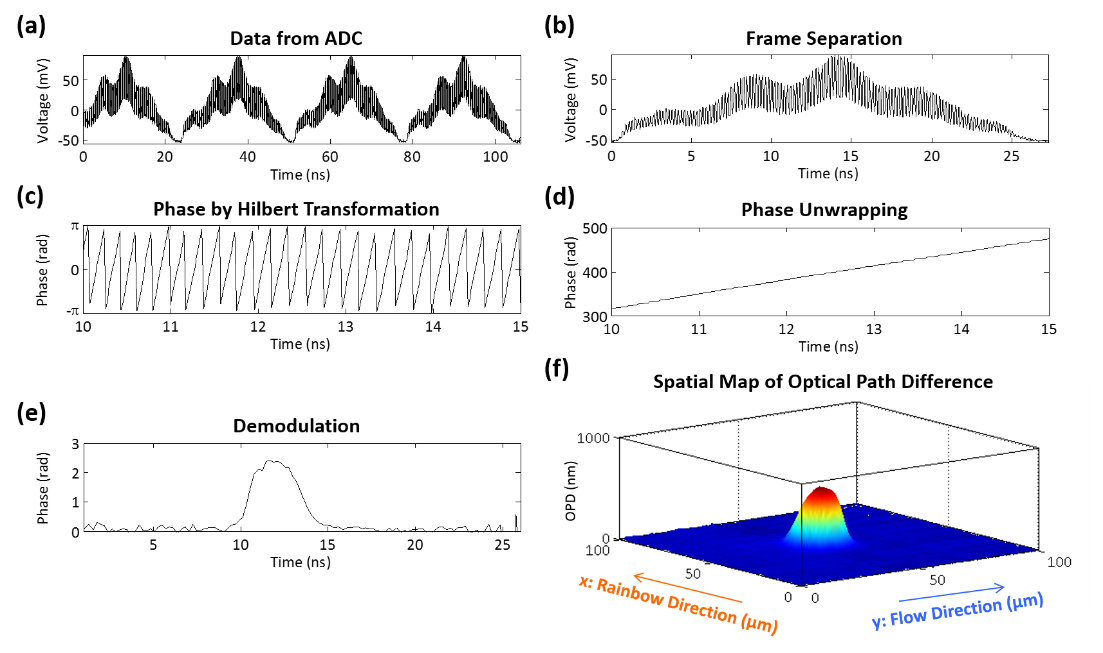
\includegraphics[scale=0.75]{BOE2013/Figure2.png}
\caption{Digital signal processing of Coherent-STEAM. (a) The photodetector output signal is digitized and recorded by an ADC. This signal shows sequential laser pulses. (b) Each pulse is saved separately as a frame for further processing. (c) The analytic form of high-frequency components of each pulse is generated using Hilbert transformation, and the phase component of this analytic form is extracted. (d) An unwrapping algorithm is used to fix unrealistic phase jumps, and the result shows an approximately linear phase increase. (e) If the phase component of the interferometer fringe frequency is removed, the phase induced by cells in optical pulse can be seen. (f) Many of these line images generated from subsequent frames are used to form a spatial map of optical path difference in two dimensions, which is used for cell characterization.}
\label{fig:BOE2013_Figure2}
\end{figure}

Spatial map of optical path difference can be used to extract the refractive index contrast between the cell and the surrounding liquid.  If the thickness of the cell at point $(x,y)$ is $t(x,y)$,
\begin{equation}
OPD(x,y) = 2 \Delta n_{cell} \cdot t(x,y)
\label{eqn:BOE2013_Equation3}
\end{equation}
where $\Delta n_{cell} = n_{cell} - n_{liquid}$ in which $n_{cell}$ and $n_{liquid}$ are the refractive indices of the cell and the surrounding liquid, respectively. The factor 2 is to account for the fact that each wavelength component passes the cell twice in Michelson interferometer. If we integrate Equation \eqref{eqn:BOE2013_Equation3} over the area of the cell, we can derive an average refractive index contrast, which corresponds to protein concentration of the cell:
\begin{equation}
\Delta n_{cell} = \frac{\iint_{cell} OPD(x,y) \ud x \ud y}{2V_{cell}}
\label{eqn:BOE2013_Equation4}
\end{equation}
where $V_{cell} = \iint_{cell} t(x,y) \ud x \ud y$ is the volume of the cell. Most of the cells relax to a spherical shape when they are released from substrates and brought into suspension \cite{revel1974adhesion,whur1977substrate}. Therefore, if we know the diameter of the cell, $d_{cell}$, we can estimate its volume as $V_{cell} \approx \pi d_{cell}^3/6$.

\section{Results and discussion}
Spherical polystyrene beads with a NIST traceable diameter of 5 $\mathrm{\mu}$m are used to calibrate the image processing algorithm for size measurements. A custom designed algorithm in CellProfiler software \cite{carpenter2006cellprofiler} is used to detect the beads or cells in spatial map of optical path difference (Figure \ref{fig:BOE2013_Figure3}). Bead or cell diameter is measured along the rainbow direction to eliminate size measurement inaccuracies caused by fluctuations of flow speed (Figure \ref{fig:BOE2013_Figure3}a). Due to limited optical resolution of the setup, the bead or cell edges are blurred, generating a small phase signal outside of the diameter bars. The diameter along the rainbow direction is equal to the diameter along the interrogation optical beam for spherical-shape beads or cells in suspension, including the samples in our experiments. 

\begin{figure}[htb!]
\centering
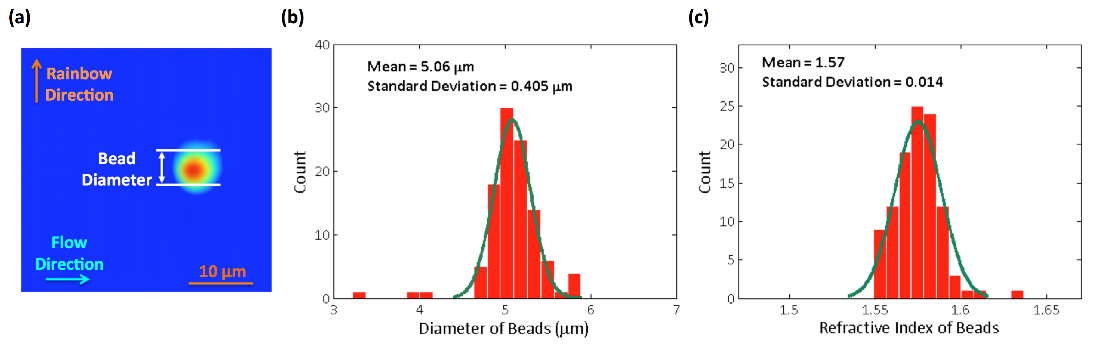
\includegraphics[scale=1]{BOE2013/Figure3.png}
\caption{Calibration with NIST traceable beads. Polystyrene beads with a NIST traceable diameter of 5 $\mathrm{\mu}$m are used to calibrate the image processing algorithm for size measurements. (a) A custom designed image processing algorithm in CellProfiler software is used to find the beads in spatial map of optical path difference and measure the diameter. (b) Histogram of bead diameters demonstrates the measured size distribution has an expected mean of 5 $\mathrm{\mu}$m and a standard deviation within the range of optical resolution limit. (c) Since all the beads are made out of the same material, the coefficient of variation for refractive indices ($0.014/1.57 = 0.89\%$) is much smaller than that of diameters ($0.405/5.06 = 8.00\%$).}
\label{fig:BOE2013_Figure3}
\end{figure}

Histogram analysis of bead diameter distribution for more than one hundred beads with corresponding Gaussian fit to measurements demonstrates that the measured size distribution has a standard deviation of 0.4 $\mathrm{\mu}$m and an expected mean of 5 $\mathrm{\mu}$m (Figure \ref{fig:BOE2013_Figure3}b). The broadening in the distribution is caused by the limited lateral optical resolution of the Coherent-STEAM setup. This resolution is measured by the knife-edge method and is about 2.5 $\mathrm{\mu}$m. Therefore, the standard deviation of the bead size distribution is well below the optical resolution.

We also measured the refractive index contrast of each bead and the surrounding liquid using Coherent-STEAM. Assuming that the refractive index of water is 1.317 at the 1581 nm to 1601 nm bandwidth, we derived the refractive index of the beads using Equation \eqref{eqn:BOE2013_Equation4}. Analysis of the bead refractive indices and corresponding Gaussian fit demonstrates that the beads have a mean refractive index of 1.57 with a standard deviation of 0.014 (Figure \ref{fig:BOE2013_Figure3}c). We observe that the coefficient of variation for the bead refractive indices is 0.89\%, which is much smaller than the coefficient of variation for the bead diameters (8.00\%). This is expected because all the beads are made out of the same material, while their diameter measurements are effected by dispersity of the size and limited spatial resolution of the setup.

We used the calibrated Coherent-STEAM setup to measure cell diameter and refractive index contrast (as a measure for protein concentration) simultaneously. Different types of cells have different mean diameters and protein concentrations; however, both of these parameters have a broad range of variations for each cell type. We see that identification of cells is more specific using both of these parameters simultaneously, instead of each individually. Images of OTII (Figure \ref{fig:BOE2013_Figure4}a) and SW480 (Figure \ref{fig:BOE2013_Figure4}b) cells taken by Coherent STEAM setup demonstrate that the cells are spherical in the microfluidic channel. In Figure \ref{fig:BOE2013_Figure4}c, scattering plot of cell protein concentration (refractive index difference) versus diameter is shown for these cells. Using points in a normal range of protein concentration and sliding the detection limit along the depicted direction (perpendicular to the optimum classification line), a receiver operating characteristic (ROC) curve is generated (Figure \ref{fig:BOE2013_Figure4}d). Comparing the ROC curve of individual parameters (e.g. size measurement only) to that of simultaneous measurement, it becomes obvious that the detection sensitivity has improved considerably. 

\begin{figure}[htb!]
\centering
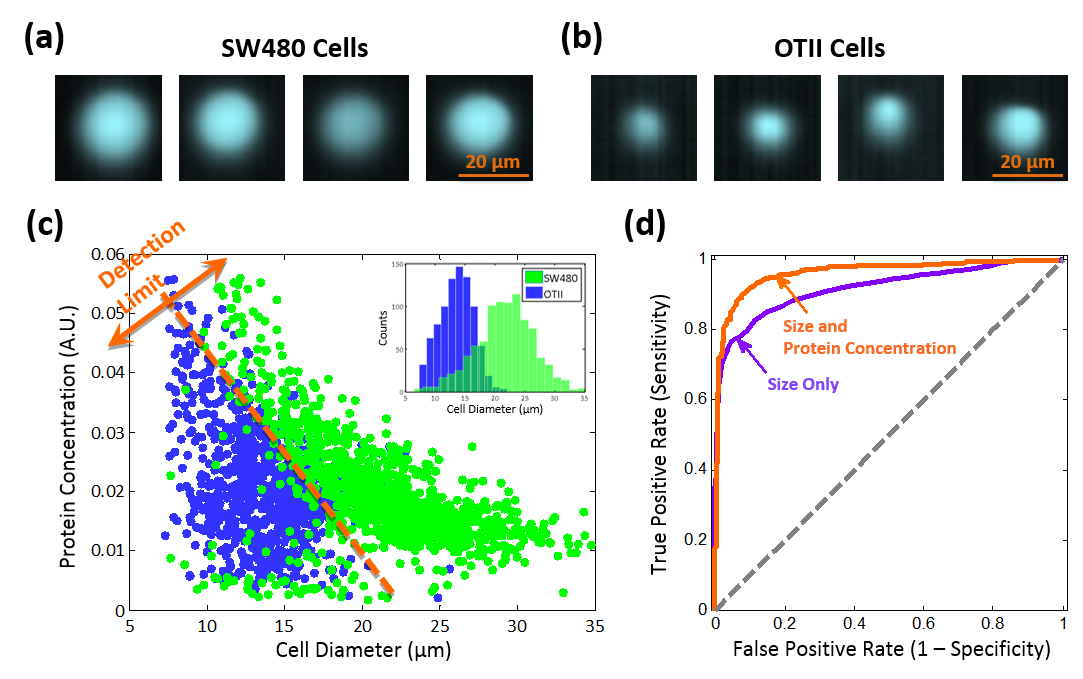
\includegraphics[scale=0.75]{BOE2013/Figure4.png}
\caption{Cell classification based on size and protein concentration measurement by Coherent-STEAM; Images of (a) SW480 and (b) OTII cells taken by Coherent STEAM setup show that they are spherical. (c) Scattering plot of cell protein concentration versus diameter is shown for OTII (blue) and SW480 (green) cells. (d) Comparison of the ROC curves of size measurement only (purple line) to that of simultaneous size and protein concentration measurement (orange line) shows significant improvement in sensitivity.}
\label{fig:BOE2013_Figure4}
\end{figure}

\section{Conclusion}

In summary, we demonstrated a new type of imaging flow cytometry based on coherent stretched-time-encoded amplified microscopy, which is capable of classifying cells in flow rates as a high as a few meters per second. Coherent-STEAM measures size and total optical path difference of cells simultaneously and extracts the refractive index, which corresponds to the protein concentration of the cells, as an additional parameter for classification. As illustrated in our experimental results, separation of two cell types was significantly enhanced by adopting the additional protein concentration parameter generated by Coherent-STEAM. We will continue our work with real-time signal processing and cell identification on field-programmable gate arrays (FPGAs) for classification of more than two cell types.

%\input {chapter4}
%\input {Conclusion}

%\bibliography {bib/network,bib/naming}    % bibliography references
%\bibliographystyle {thesis}

%\bibliographystyle {IEEEtran}
%\bibliography {IEEEfull,DissertationBib} 

\bibliography{DissertationBib}
\bibliographystyle{unsrt}

\end {document}
